\documentclass{tufte-handout}
\usepackage{amsmath,amsthm}

\input{vc.tex}

\usepackage{pgfplots}
\pgfplotsset{width=\textwidth,compat=1.5.1}

\newtheorem{claim}{Claim}[section]
\title{\sf Pagerank}
%\date{\GITAuthorDate}
%\author{Thore Husfeldt}

\begin{document}
\maketitle
\footnotetext{rev. \GITAbrHash}

\section{Pagerank}

\begin{marginfigure}
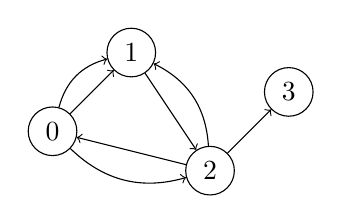
\begin{tikzpicture}
\node (0) [draw,circle] at (0,0) {0};
\node (1) [draw,circle] at (1,1) {1};
\node (2) [draw,circle] at (2,-.5) {2};
\node (3) [draw,circle] at (3,.5) {3};
\draw [->] (0) to [bend left] (1);
\draw [->] (0) to  (1);
\draw [->] (0) to [bend right] (2);
\draw [->] (1) to  (2);
\draw [->] (2) to  (0);
\draw [->] (2) to [bend right] (1);
\draw [->] (2) to (3);
\end{tikzpicture}
\caption{A directed multigraph.}
\end{marginfigure}
Consider an finite, directed multigraph $G=(V,E)$ without self-loops, as in
Fig.~1.
We will understand $G$ as the hyperlink structure of the web pages
described by $V$; an arc from vertex $u$ to vertex $v$ describes a
hyperlink from page $u$ to page $v$.

The \emph{random surfer} model is a stochastic process that aims to
rank the relevance of a these pages.
The states of this process are the vertices $V$.
With good probability $\alpha$, the process picks an outgoing edge at
random and moves to that page.
If there are no outgoing edges, the surfer picks a random page from
$V$ instead.
(Note that outgoing edges are counted with multiplicities, so from
vertex~0 in the example, the chance of going to 1 is twice that of
going to 2.)
Alternatively, with probability $(1-\alpha)$, the surfer becomes bored
and moves to a random page from $V$ instead.
The probability $\alpha$ is called the \emph{damping factor}; a
typically value that works well for web pages is $\alpha = \frac{85}{100}$. 

This process is a finite, irreducible, and ergodic Markov chain.
Its stationary distribution describes the \emph{page rank} of each
vertex. The contribution of Sergey Brin and Larry Page was to
realise that this value gives a good measure of the relevance of a web
page, which is the main idea behind the search engine
Google.

\subsection{Files}


\begin{marginfigure}
\begin{verbatim}
4
0 1   0 1   0 2
1 2   
2 0   2 1
2 3
\end{verbatim}
\caption{Input file for the graph in Fig.~1.}
\end{marginfigure}

Vertex names are integers $V= \{0,\ldots, n-1\}$.
Input files contain $|V|$, followed by $u$ and $v$ for each $(u,v)\in
E$.
The files are in the data directory are:
\begin{quotation}
\begin{description}
\item[three.txt] The 4-vertex graph from Fig.~1.
\item[tiny.txt] The 5-vertex graph from \S{}1.6 from Sedgewick and
  Wayne.\sidenote{R. Sedgewick and K. Wayne,
  \emph{Programming in Java: An Interdisciplinary Approach}, Addison
  Wesley, 2007.}
\item[medium.txt] The 50-vertex graph \emph{ibid.}
\item[wikipedia.txt] The 11-vertex graph from Wikipedia's PageRank article.\sidenote{``PageRank.'' Wikipedia, The Free Encyclopedia. Wikimedia
  Foundation, Inc. Accessed 16 Sep 2012.}
\item[p2p-Gnutella08-mod.txt] A 6301-vertex graph describing a file
  sharing network. 
Vertices represent hosts in the Gnutella network topology and edges
represent connections between the Gnutella host, collected 8 August
2002.\sidenote{Modified from the Stanford University SNAP library,
  original file at
  snap.stanford.edu/data/p2p-Gnutella08.html. Sources:
J. Leskovec, J. Kleinberg and C. Faloutsos. \emph{Graph Evolution: Densification and Shrinking Diameters}. ACM Transactions on Knowledge Discovery from Data (ACM TKDD), 1(1), 2007.
M. Ripeanu and I. Foster and A. Iamnitchi. \emph{Mapping the Gnutella
  Network: Properties of Large-Scale Peer-to-Peer Systems and
  Implications for System Design}. IEEE Internet Computing Journal,
2002.}
\end{description}
\end{quotation}

\subsection{Deliverables}

\begin{enumerate}
\item Implement a simulation of the random surfer model. 
  Start in
  vertex 0 and follow the rules for a given number of iterations read
  from the command line. Count the number of times each vertex is
  visited and print the relative frequencies.
\item Solve the exact same problem using linear algebra instead of
  simulation.
  That is, construct the transition probability matrix $P$ and
  compute $pP^r$ for some sufficiently high $r$ (read from the command
  line) and some initial vector $p$ of your choice.
  In fact, we're approximating the dominant left eigenvector, i.e., a
  vector satisfying $pP= p$.
  There are (at least) 3 ways of computing $pP^r$:
  \begin{enumerate} 
  \item Let $p_0= p$. For each $i=1,\ldots, m$ let $p_i = p_{i-1}
    P$. Return $p_r$.
  \item Compute $Q = P^r = P\cdot P \cdots P$ using $r-1$ matrix products.
    Return $pQ$.
  \item Compute $P^r$ by iterated squaring. Assume $r$ is a power of
    2. Set $Q_0 = P$ and for $i=1,\ldots,\log r$ compute $Q_i =
    Q_{i-1}^2$. Return $pQ_{\log r}$. 
  \end{enumerate}
  Pick the one you think is fastest or easiest to implement for the
  small instances.

  However, to attack an instance of nontrivial size, you need to
  exploit the structure of the transition matrix.
  (Unless you like waiting a lot.)
  Let $A$ denote the adjacency matrix of $G$, and define the two
  matrices
  \[
  H_{ij} =
  \begin{cases}
    A_{ij} / \deg(i)\,, & \text{if } \deg(i) > 0\,; \\
    0\,, & \text{if } \deg(i) = 0 \,;   
  \end{cases}
  \]
  and
  \[
  D_{ij} =
  \begin{cases}
    0\,, & \text{if } \deg(i) > 0\,; \\
    1 / n\,, & \text{if } \deg(i) = 0\,.
  \end{cases}
  \]
  Then,
  \[ P = \alpha(H + D) + \frac{1-\alpha}{n} \bf 1\,,\]
  where $\bf 1$ is the $|V|\times |V|$ all-1s matrix.
  In particular,
  \[pP = \alpha p H + \alpha p D + \frac{1-\alpha}{n} p \bf 1\,.\] All
  three of these vector--matrix products are simpler to compute: all
  columns in $D$ are identical, all columns in $\bf 1$ are identical,
  and $H$ is sparse (so you don't store is as a square matrix of size
  $O(|V|^2)$; just as a list of $O(|E|)$ nonzero values).
  Oh, and if you really just wrote code to compute the dot product
  between $p$ and an all-1s vector, this is a good time for a break.
\item Fill out the report.
\end{enumerate}


\newpage
\section{Pagerank Lab Report}


by Anton Friberg

\subsection{Transition probabilities}

The transition matrix for the graph described in three.txt
is\sidenote{Fill in the right values. Set $\alpha=\frac{85}{100}$.}
\begin{equation*}
P = 
\left(
\begin{array}{cccc}
0.04 & 0.60 & 0.32 & 0.04 \\
0.04 & 0.04 & 0.89 & 0.04 \\
0.32 & 0.32 & 0.04 & 0.32 \\
0.25 & 0.25 & 0.25 & 0.25 \\
\end{array}
\right)\,,
\end{equation*}
and its 10th power is
\begin{equation*}
P^{10} = 
\left(
\begin{array}{cccc}
0.18 & 0.28 & 0.36 & 0.18 \\
0.18 & 0.28 & 0.36 & 0.18 \\
0.18 & 0.28 & 0.36 & 0.18 \\
0.18 & 0.28 & 0.36 & 0.18 \\
\end{array}
\right)\,.
\end{equation*}

The transition matrix $P$ can be broken down into  $P = \alpha(H + D)
+ \frac{1-\alpha}{n} \bf 1$, where
\begin{equation*}
H =
\left(
\begin{array}{cccc}
0.00 & 0.67 & 0.33 & 0.00 \\
0.00 & 0.00 & 1.00 & 0.00 \\
0.33 & 0.33 & 0.00 & 0.33 \\
0.00 & 0.00 & 0.00 & 0.00 \\
\end{array}
\right)\,.
\end{equation*}
and \begin{equation*}
D =
\left(
\begin{array}{cccc}
0.00 & 0.00 & 0.00 & 0.00 \\
0.00 & 0.00 & 0.00 & 0.00 \\
0.00 & 0.00 & 0.00 & 0.00 \\
0.25 & 0.25 & 0.25 & 0.25 \\
\end{array}
\right)\,.
\end{equation*}

\subsection{Results}

The following table gives the top hits, i.e., the 5 first vertices of
each graph sorted by page rank, using $\alpha = \frac{85}{100}$.

\medskip
\begin{fullwidth}
\small
\begin{tabular}{lcccccccccc}
three.txt & 2 (36.4\%) & 1 (27.9\%) & 0 (17.9\%) & 3 (17.9\%) \\
tiny.txt & 0 (27.7\%) & 3 (25.4\%) & 1 (24.5\%) & 2 (15.1\%) & 4 (7.3\%) \\
medium.txt & 22 (5.7\%) & 6 (5.6\%) & 13 (3.8\%) & 28 (3.7\%) & 23 (3.6\%) \\
wikipedia.txt & 1 (43.3\%) & 2 (32.2\%) & 4 (6.5\%) & 3 (3.4\%) & 5 (3.4\%) \\
p2p-Gnutella08-mod.txt & 367 (0.34\%) & 5 (0.30\%) & 1317 (0.30\%) & 249 (0.28\%) & 145 (0.28\%) \\
\end{tabular}
\end{fullwidth}

\medskip
Note that p2p-Gnutella08-mod.txt is a $(6301x6301)$ size matrix. As each multiplication takes $6301^3 = 250166088901$
operations the compute time of $P^{10}$ was several minutes.

\bigskip The following table gives the number of random walk steps and
(scalar) multiplications needed for each graph until the results were
stable to within 2 decimal places.

\medskip
\begin{fullwidth}
\small
\begin{tabular}{lcccccccccc}
Graph & \# transitions  & \# multiplications \\
three.txt & 6,663 \\
tiny.txt  & 7,563 \\
medium.txt & 10,064\\
wikipedia.txt & 6,503 \\
p2p-Gnutella08-mod.txt & 10,530
\end{tabular}
\end{fullwidth}

\subsection{Optional}

Build a time machine, fly back to the early 1990s.
Start a search engine company based on this idea.


\section{Perspective}

For more thorough introduction to the mathematics
  behind this model, see David Austin, \emph{How Google Finds Your Needle in
  the Web's Haystack}, American Mathematical Society Feature Column,
  2006.\sidenote{www.ams.org/samplings/feature-column/fcarc-pagerank, retrieved
20 Sep 2012.}

The original paper is Sergey Brin, Lawrence Page, \emph{The anatomy of a
large-scale hypertextual Web search engine}\sidenote{Computer Networks
  and ISDN Systems, 33: 107-17, 1998.
  infolab.stanford.edu/pub/papers/google.pdf}, which also mentions a
bit about the data structure used for storing web page content.
A different model for establishing web page relevance was established
by Kleinberg around the same time as PageRank.\sidenote{Kleinberg, Jon (1999).
  \emph{Authoritative sources in a hyperlinked environment}.
  Journal of the ACM 46 (5): 604--632.
  doi:10.1145/324133.324140.}
\end{document}
